\documentclass[11pt]{article}
\usepackage[a4paper,margin=1in]{geometry}
\usepackage[T1]{fontenc}
\usepackage[utf8]{inputenc}
\usepackage{lmodern}
\usepackage{microtype}
\usepackage{amsmath,amssymb,amsthm,mathtools}
\usepackage{booktabs,array,float,placeins,enumitem}
\usepackage{graphicx,xcolor}
\usepackage{tikz}
\usetikzlibrary{arrows.meta,positioning,calc,fit,backgrounds,shapes.geometric}
\usepackage[numbers,super,sort&compress]{natbib}
\usepackage{caption}
\DeclareCaptionLabelSeparator{nhbbar}{ $|$ }
\captionsetup{labelfont=bf,labelsep=nhbbar,font=small}
\renewcommand{\figurename}{Fig.}
\usepackage{setspace}
\usepackage{hyperref}
\hypersetup{colorlinks=true,citecolor=blue,linkcolor=blue,urlcolor=blue}
\setstretch{1.08}
\setlength{\emergencystretch}{3em}
\raggedbottom
\graphicspath{{figures/}}
\setcounter{secnumdepth}{0}

\newcommand{\E}{\mathbb{E}}
\newcommand{\Prob}{\mathbb{P}}
\newcommand{\1}{\mathbf{1}}
\newcommand{\Astar}{A^{*}}
\definecolor{verm}{HTML}{D55E00}
\definecolor{blu}{HTML}{0072B2}

\title{\bfseries Reference-dependent delegitimation:\\ cognitive dissonance turns collective failure into self-defending error}
\author{Gabriel Bontemps$^{1,2,3,\ast}$ \and Abhishek Banerjee$^{2,3}$}
\date{\small $^1$GREDEG-CNRS, Universit\'e C\^ote d'Azur, Nice, France. $^2$Blizard Institute, Queen Mary University of London, UK. $^3$Adaptive Decisions Laboratory, Department of Pharmacology, University of Oxford, UK.\\ $^\ast$e-mail: g.l.s.bontemps@qmul.ac.uk\\[2mm] Working manuscript (simulation study) --- \today}

\begin{document}
\maketitle

\begin{abstract}
\noindent People who fail repeatedly often stop asking what they did wrong and start asking whether the game is fair. We build a theory in which both reactions flow from one source: a single cognitive-dissonance objective whose two gradients are reinforcement learning gated by legitimacy, and the erosion of legitimacy itself. Its central result is \emph{reference-dependent delegitimation}: outcomes lose their authority as evidence only when they fall short of what the agent has learned to feel entitled to---never on failure alone. In simulations, networked communities that keep losing while winners stay visible lock onto wrong actions and reject the evidence that would correct them (probability $0.843$ at a pre-declared cell and horizon; a designed validation, not a discovery). The trap obeys one law at any number of communities, tested from two to ten thousand: a community's structural exposure to corrected communities sets the edges of a window and its two clocks, and community size decides inside it. Making success visible heals every Bayesian rival we instantiate at the speed of evidence; dissonant agents correct what they do yet keep their grievance---so the theory derives when echo chambers discredit outside evidence, rather than assuming that they do. Reference-dependent delegitimation is the single confirmatory target of the accompanying preregistration-ready experiment.
\end{abstract}

\vspace{2mm}

\section{Introduction}

A bad outcome is ambiguous evidence. It can mean that one's belief about the best action was wrong, or that the rule assigning outcomes is not worth learning from. Nearly all formal theories of individual and social learning resolve the ambiguity by assumption: realized rewards are evidence about actions, and prediction errors discipline beliefs\cite{SuttonBarto2018,DeGroot1974,GolubJackson2010}. A long behavioural tradition documents the second reading---people discount or reject feedback that conflicts with what they feel entitled to\cite{Festinger1957,Kunda1990,Tyler2006}---and it has now reached the reward-learning laboratory: disadvantageous inequity degrades stimulus--reward learning even at constant own payoffs\cite{HamJenkins2025}. The question this paper answers is when a group that keeps losing stops learning and starts disbelieving---and why showing it the winners heals what it does while hardening what it believes.

Here we derive the second reading instead of assuming it, and follow its consequences through a network. After enough failure, an agent's effective problem is no longer maximizing reward but minimizing dissonance: revise beliefs about actions, or revise belief in the game. One per-period dissonance functional over those two cognitions---action values $Q$ and the legitimacy $L$ granted to the reward rule as evidence---returns, gradient by gradient, reinforcement learning gated by legitimacy (the effective prediction error is $L\delta$) and threshold delegitimation (legitimacy erodes when outcomes fall intolerably short of an entitlement benchmark, and recovers when they are acceptable). Reward-maximizing learning is the corner of the same problem in which frame revision is unavailable: the ``switch'' to self-justification is a reallocation within one objective, governed by the agent's own history (Methods; a non-lexicographic variant adds a surprise-erosion term and is tested alongside).

The benchmark is where the theory earns its keep. Entitlement is an adaptive aspiration---a recency-weighted average of one's own outcomes, anchored to the visible outcomes of others\cite{Simon1955,Selten1998,KoszegiRabin2006}, with the asymmetric sting of inequity aversion\cite{FehrSchmidt1999}---and the gate closes only when aspiration exceeds a critical level $\Astar$: failure never delegitimizes; failure relative to what one still feels entitled to does. We call this \emph{reference-dependent delegitimation}; it is the paper's central object, and the one prediction the accompanying experiment is designed to confirm.\footnote{The slogan is a property of the lexicographic convention as much as of the functional: the non-lexicographic variant, in which surprise itself erodes legitimacy, partially traps even at neutral entitlement ($P=0.257$ against $0.000$; Supplementary Section~S12)---the convention is load-bearing and empirically distinguishable rather than innocuous.} When aspiration is purely self-referential, grievance burns itself out: aspirations sink to match experience---Elster's sour grapes\cite{Elster1983}. Lasting delegitimation therefore needs an anchor that refuses to adapt: visible unequal success (fraternal relative deprivation\cite{Runciman1966,Gurr1970,SmithPettigrew2012}), a cultural constant, or sheer slowness. Whether a population is trapped at all comes down to a race between legitimacy collapsing and aspiration adapting, with a closed-form critical rate; the algebraic skeleton is machine-verified in Lean~4\cite{MoultonLean}.

Collectively, agents interact on a network in which confidence-weighted choices circulate and feed back into decisions---a reputation-like summary statistic\cite{AxelrodHamilton1981}. Early luck can lock a community onto the wrong action; grievance then gates learning, and that is what can make a collective error self-defending. The nearest rational accounts make wrong beliefs self-confirming\cite{HeidhuesKoszegiStrack2018,EspondaPouzo2016,Bohren2016,BohrenHauser2021,FrickIijimaIshii2020}; the economics of dissonance makes beliefs objects of choice\cite{AkerlofDickens1982,Rabin1994,Benabou2013}; grievance models of unrest work through protest thresholds\cite{Epstein2002}. Here, instead, the world-model is right, nothing is chosen, and only the \emph{weighting} of evidence is motivated: the gate is a myopic gradient step, entitlement a learned state, and deprivation acts on the evidential status of feedback. The equilibrium notion is self-confirming\cite{FudenbergLevine1993}, the metastable dwell and slow-clock escape familiar from adaptive learning in macroeconomics\cite{EvansHonkapohja2001,ChoWilliamsSargent2002}---the escape here carried by aspiration. Collective-failure theory sharpens the contrast: cascades and naive pooling fail at \emph{supply}---actions conceal signals, or influence is unbalanced\cite{Banerjee1992,BikhchandaniHirshleiferWelch1992,DeGroot1974,GolubJackson2010}; bounded-confidence dynamics move weights with opinion distance\cite{HegselmannKrause2002}; the echo-chamber literature names, but does not derive, the active discrediting that distinguishes a chamber from a bubble\cite{Nguyen2020,Cinelli2021}. Here the discrediting is derived from outcome histories alone, and the model predicts when cross-cutting exposure corrects and when it entrenches---the pattern field experiments keep finding\cite{Bail2018}. And the comparison with rational rule-suspicion is run below, not asserted.

Our contribution is fourfold: the theory of reference-dependent delegitimation (the critical aspiration $\Astar$, a resignation proposition, a relative-deprivation condition, a closed-form critical adaptation rate); the as-if representation behind it, whose content is the coupling it imposes---one legitimacy state across both margins, loss and repair mutually exclusive within a period ($X_tK_t=0$), erosion graded while repair capped, one cost ratio spanning the continuum from pure reward learning to pure self-justification---none of which two free-standing postulates about motivated discounting\cite{Festinger1957,Kunda1990} would impose; the collective results---a frozen-design confirmatory experiment, regime maps realizing four social fates in one plane, the transparency dissociation, and the trap's structural scope conditions; and a measurement doctrine fixing what an empirical test can recover and which model-free signatures must therefore carry the burden. The full audit trail---designs frozen before execution, negative results with their counterexamples---lives in the Supplement and the repository.

\begin{figure}[t]
\centering
\resizebox{\textwidth}{!}{%
% TikZ conventions (box lanes, flow/gate/soc arrow styles, the red "gates evidence"
% arrow, fairness lane, regime-map cell layout with high/low axis ticks) are adapted
% from the authors' working-paper TikZ sources supplied with the project archives:
%   WP2--draft1/figures/fig1_mechanism.tex  and  WP2--draft1/figures/fig_regimemap.tex
% (also WP1_arxiv_package/figures/fig1_mechanism.tex); cell tints are remapped to this
% paper's CVD-validated palette so Fig.~1b matches the empirical regime-map figure.
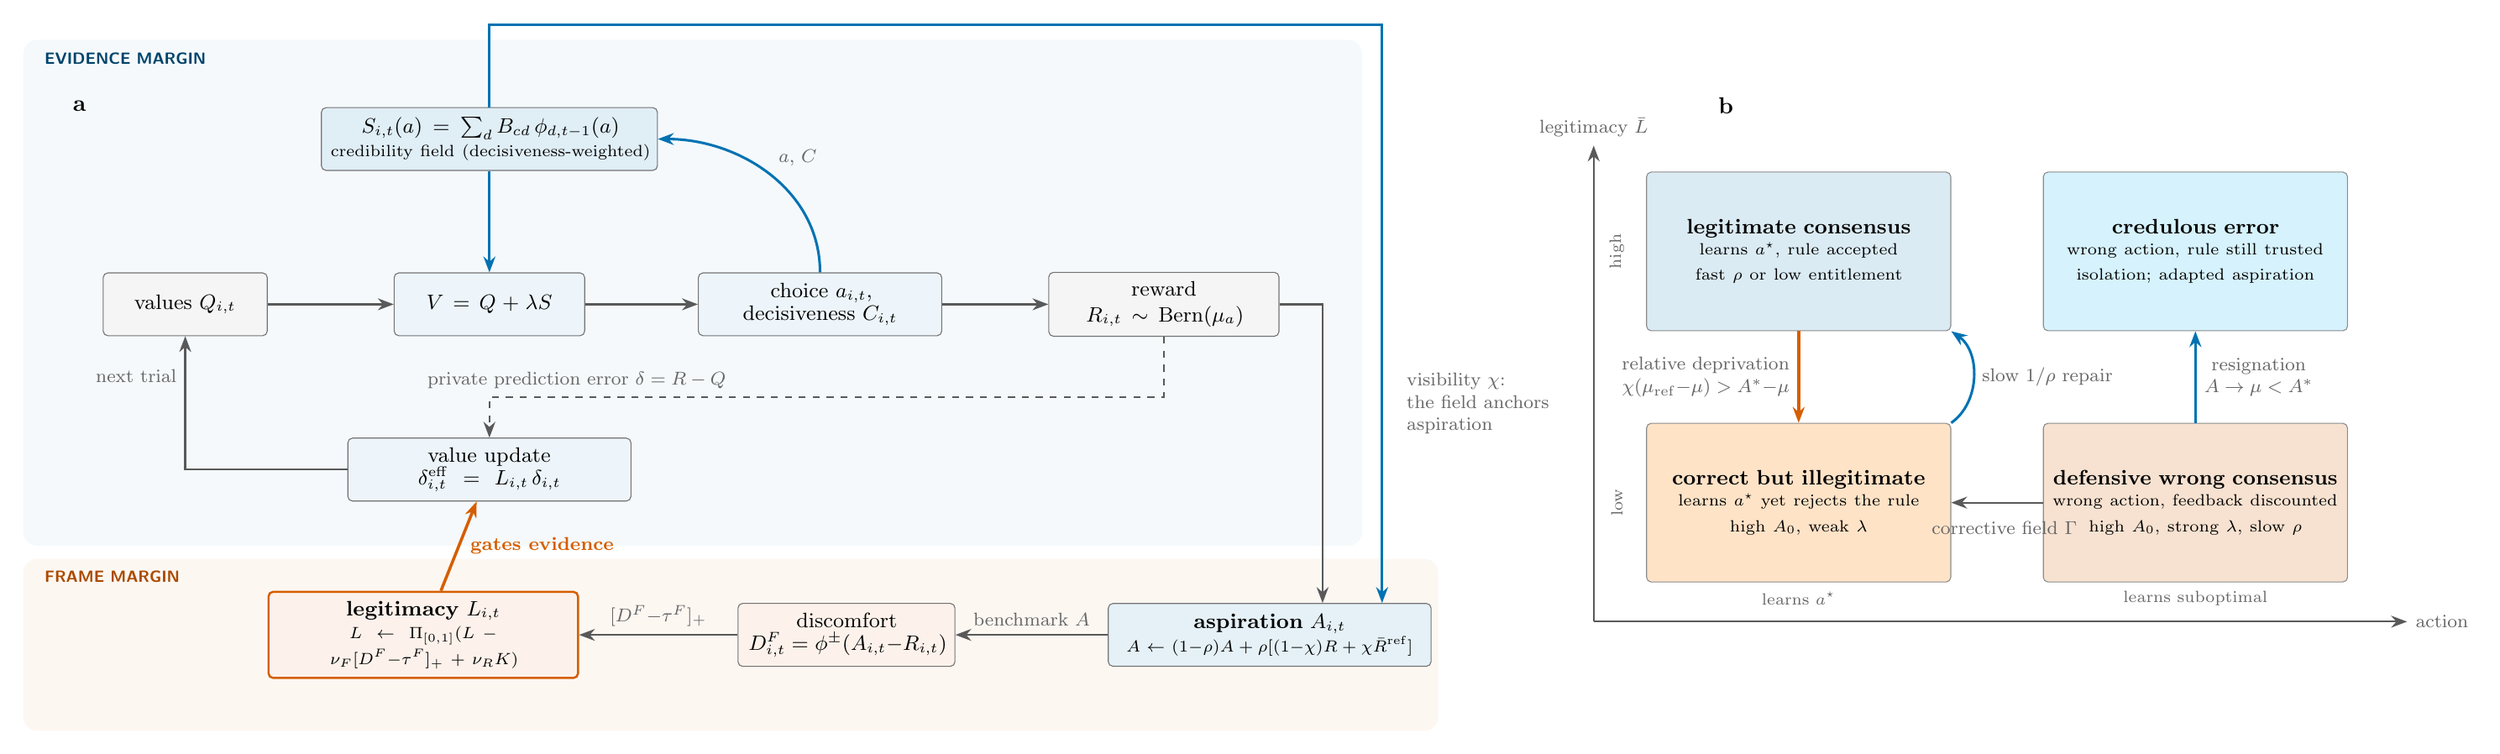
\begin{tikzpicture}[
  font=\small, >={Stealth[length=2.4mm]},
  box/.style={draw=black!55, rounded corners=2pt, align=center, minimum height=9.5mm, inner sep=4pt},
  state/.style={box, fill=black!4},
  proc/.style={box, fill=blu!7},
  fair/.style={box, fill=verm!8},
  flow/.style={->, thick, black!65},
  gate/.style={->, line width=1.3pt, verm},
  soc/.style={->, line width=1.1pt, blu},
  lbl/.style={font=\footnotesize, black!60, align=center}]
% ===== panel a: mechanism (lane layout after WP fig1_mechanism) =====
\begin{scope}[on background layer]
\fill[blu!4, rounded corners=6pt] (-2.45,-3.65) rectangle (17.8,4.0);
\fill[verm!5, rounded corners=6pt] (-2.45,-6.45) rectangle (18.95,-3.85);
\node[font=\scriptsize\sffamily\bfseries, text=blu!60!black, anchor=west] at (-2.25,3.72) {EVIDENCE MARGIN};
\node[font=\scriptsize\sffamily\bfseries, text=verm!80!black, anchor=west] at (-2.25,-4.12) {FRAME MARGIN};
\end{scope}
\node[font=\bfseries] at (-1.6, 3.0) {a};
\node[box, fill=blu!12, text width=48mm] (S) at (4.6, 2.5)
  {$S_{i,t}(a)=\sum_d B_{c d}\,\phi_{d,t-1}(a)$\\[-1pt]\scriptsize credibility field (decisiveness-weighted)};
\node[state, text width=22mm] (Q)  at (0.0,0)  {values $Q_{i,t}$};
\node[proc, text width=26mm]  (V)  at (4.6,0)  {$V=Q+\lambda S$};
\node[proc, text width=34mm]  (CH) at (9.6,0)  {choice $a_{i,t}$,\\[-1pt] decisiveness $C_{i,t}$};
\node[state, text width=32mm] (R)  at (14.8,0) {reward $R_{i,t}\sim\mathrm{Bern}(\mu_a)$};
\node[proc, text width=40mm] (UPD) at (4.6,-2.5) {value update\\[-1pt] $\delta^{\mathrm{eff}}_{i,t}=L_{i,t}\,\delta_{i,t}$};
\node[fair, draw=verm, line width=.9pt, text width=44mm] (L) at (3.6,-5.0)
  {\textbf{legitimacy} $L_{i,t}$\\[-1pt]\scriptsize $L \leftarrow \Pi_{[0,1]}(L-\nu_F[D^F{-}\tau^F]_+ +\nu_R K)$};
\node[fair, text width=30mm] (DF) at (10.0,-5.0) {discomfort\\[-1pt] $D^F_{i,t}=\phi^{\pm}(A_{i,t}{-}R_{i,t})$};
\node[box, fill=blu!10, text width=46mm] (ASP) at (16.4,-5.0)
  {\textbf{aspiration} $A_{i,t}$\\[-1pt]\scriptsize $A\leftarrow(1{-}\rho)A+\rho[(1{-}\chi)R+\chi\bar R^{\mathrm{ref}}]$};
\draw[flow] (Q) -- (V);
\draw[flow] (V) -- (CH);
\draw[flow] (CH) -- (R);
\draw[soc]  (S) -- (V);
\draw[soc]  (CH.north) to[out=90,in=0] node[above right, lbl, pos=.5]{$a,\,C$} (S.east);
\draw[flow, dashed] (R.south) |- (7.6,-1.4) -| (UPD.north)
  node[pos=.28, above, lbl]{private prediction error $\delta=R-Q$};
\draw[flow] (UPD.west) -| node[left, lbl, pos=.85]{next trial} (Q.south);
\draw[flow] (R.east) -| ([xshift=8mm]ASP.north);
\draw[soc]  (S.north) -- ++(0,1.25) -| ([xshift=17mm]ASP.north);
\node[lbl, align=left, anchor=west] at (18.35,-1.5) {visibility $\chi$:\\ the field anchors\\ aspiration};
\draw[flow] (ASP) -- node[above, lbl]{benchmark $A$} (DF);
\draw[flow] (DF) -- node[above, lbl]{$[D^F{-}\tau^F]_+$} (L);
\draw[gate] (L) -- node[right=1pt, font=\footnotesize\bfseries, verm]{gates evidence} (UPD);
% ===== panel b: regime map (cells after WP fig_regimemap; palette = empirical map) =====
\begin{scope}[shift={(24.4,-6.6)}]
\node[font=\bfseries] at (-1.1, 9.6) {b};
\tikzset{cell/.style={minimum width=46mm, minimum height=24mm, align=center,
         draw=black!45, rounded corners=2pt, text width=43mm}}
\node[cell, fill=blu!14]  (LC) at (0,7.4)   {\textbf{legitimate consensus}\\[1pt]\scriptsize learns $a^\star$, rule accepted\\ \scriptsize fast $\rho$ or low entitlement};
\node[cell, fill=cyan!16] (CE) at (6.0,7.4) {\textbf{credulous error}\\[1pt]\scriptsize wrong action, rule still trusted\\ \scriptsize isolation; adapted aspiration};
\node[cell, fill=orange!22] (CI) at (0,3.6) {\textbf{correct but illegitimate}\\[1pt]\scriptsize learns $a^\star$ yet rejects the rule\\ \scriptsize high $A_0$, weak $\lambda$};
\node[cell, fill=verm!18] (DW) at (6.0,3.6) {\textbf{defensive wrong consensus}\\[1pt]\scriptsize wrong action, feedback discounted\\ \scriptsize high $A_0$, strong $\lambda$, slow $\rho$};
\draw[->,thick,black!65] (-3.1,1.8) -- (-3.1,9.0) node[above, lbl]{legitimacy $\bar L$};
\node[rotate=90, font=\scriptsize, black!60] at (-2.75,7.4){high};
\node[rotate=90, font=\scriptsize, black!60] at (-2.75,3.6){low};
\draw[->,thick,black!65] (-3.1,1.8) -- (9.2,1.8) node[right, lbl]{action};
\node[font=\scriptsize, black!60] at (0,2.15){learns $a^\star$};
\node[font=\scriptsize, black!60] at (6.0,2.15){learns suboptimal};
\draw[gate] (LC.south) -- node[left, lbl]{relative deprivation\\ $\chi(\mu_{\mathrm{ref}}{-}\mu)>\Astar{-}\mu$} (CI.north);
\draw[soc]  (DW.north) -- node[right, lbl]{resignation\\ $A\to\mu<\Astar$} (CE.south);
\draw[flow] (DW.west) -- node[below, lbl, yshift=-1.5mm, pos=.42]{corrective field $\Gamma$} (CI.east);
\draw[soc]  (CI.north east) to[out=35,in=325] node[right, lbl]{slow $1/\rho$ repair} (LC.south east);
\end{scope}
\end{tikzpicture}}%
\caption{\textbf{One dissonance functional, two margins, four regimes.} \textbf{a}, Each reward feeds two conflicts of one functional (equation~\eqref{eq:D}): the evidence conflict updates action values through the legitimacy gate ($\delta^{\mathrm{eff}}=L\delta$), and the entitlement conflict is measured against an aspiration that adapts to own outcomes and anchors to visible others'. Choices circulate on a two-community network and feed back into decisions. \textbf{b}, Being right and accepting the rule are independent axes; the derived mechanisms (resignation, relative deprivation, corrective field, slow repair) move populations between the four regimes.}
\label{fig:mech}
\end{figure}

\section{Results}

\subsection{Both reactions to failure are gradients of one dissonance functional}

After choosing an action and receiving a reward, an agent holds two discrepancies at once. The evidence conflict is the prediction error $\delta_t=R_t-Q_t(a_t)$. The entitlement conflict is the gap between the reward and the agent's aspiration $A_t$, felt asymmetrically---shortfalls sting more than windfalls please: $D^F_t=\phi^-[A_t-R_t]_+ + \phi^+[R_t-A_t]_+$ with $\phi^->\phi^+$. Discomfort beyond a tolerance $\tau^F$ is the excess $X_t=[D^F_t-\tau^F]_+$; an outcome within tolerance is acceptable, $K_t=\1\{D^F_t\le\tau^F\}$. The per-period dissonance over the two revisable cognitions $(Q,L)$ is
\begin{equation}
\mathcal D(Q,L)=\underbrace{\tfrac{L}{2}\big(R_t-Q(a_t)\big)^2}_{\text{evidence conflict}}+\;w_f\underbrace{\big[L X_t+(1-L)\kappa K_t\big]}_{\text{frame conflict}}.
\label{eq:D}
\end{equation}
Each term prices a way of being wrong: a reward--belief discrepancy is dissonant only insofar as the rule is held legitimate ($L$ is the importance weight on evidence); holding the rule legitimate under intolerable deprivation is dissonant; and so is holding a grievance while outcomes are acceptable, at maintenance ratio $\kappa>0$ (Methods). By construction $X_tK_t=0$: loss and repair never fire on the same trial, which is what makes the increment asymmetry measured below a signature rather than an artefact. Gradient steps, margin by margin, give exactly
\begin{equation}
Q_{t+1}(a_t)=Q_t(a_t)+\alpha L_t\delta_t,\qquad
L_{t+1}=\Pi_{[0,1]}\big(L_t-\nu_F X_t+\nu_R K_t\big),
\label{eq:updates}
\end{equation}
---legitimacy-gated reinforcement learning and a threshold legitimacy dynamic ($\Pi_{[0,1]}$ projects onto $[0,1]$), the two margins of one stated objective (Methods; the underlying identities are machine-checked\footnote{Seven Lean~4 theorems (v4.28.0, core library only, over $\mathbb Q$) certify the algebraic core: the gradient-derivation identity behind equation~\eqref{eq:updates}, the $\Astar$ equivalences with their expectation bridge---certifying $\E[\Delta L]>0\iff A<\Astar$ in the generic region---benchmark-gap decay, and the gated contraction with its $n$-step form; axiom closure exactly \{\texttt{propext}, \texttt{Classical.choice}, \texttt{Quot.sound}\}, no \texttt{sorry}. The formal layer certifies algebra only. Statements and scope: Supplementary Section~S7; sources and verification logs: \texttt{github.com/TrompetteMarine/CSL} and \texttt{CSL2}, branch \texttt{lean-diss-core}.}). The corners: with frame revision unavailable ($\nu_F=\nu_R=0$, $L\equiv1$), a standard reward-maximizing learner; with $\alpha=0$, a pure self-justifier that never learns. The derivation is deliberately myopic---forward-looking belief management\cite{BenabouTirole2002,Benabou2016} is excluded by construction. Entitlement, finally, is endogenous: $A_{t+1}=(1-\rho)A_t+\rho[(1-\chi)R_t+\chi\bar R^{\mathrm{ref}}_t]$, adapting at rate $\rho$ and anchored with weight $\chi$ to visible reference outcomes (Fig.~\ref{fig:mech}a).

\subsection{Entitlement, not failure, closes the gate}

On an arm with success probability $\mu$, the expected legitimacy drift is $\E[\Delta L]=-\nu_F(1-\mu)(\phi^-A-\tau^F)+\nu_R\mu$ in the generic region, which is negative precisely when aspiration exceeds
\begin{equation}
\Astar(\mu)=\frac{\tau^F+(\nu_R/\nu_F)\,\mu/(1-\mu)}{\phi^-}
\label{eq:astar}
\end{equation}
(Fig.~\ref{fig:theory}a; machine-checked). Three consequences organize everything that follows. \emph{Resignation.} With self-referential aspiration ($\chi=0$), aspiration sinks to match experience, $A_t\to\mu$. Whenever $\mu<\Astar(\mu)$ the drift turns positive in finite time: grievance burns out and the gate reopens (Fig.~\ref{fig:theory}b). Adaptive-preference formation\cite{Elster1983} thus emerges from the same functional, doubling as the account of quiescence under shared hardship\cite{JostBanajiNosek2004}. \emph{Relative deprivation.} With anchoring $\chi>0$ to a reference earning $\mu_{\mathrm{ref}}$, the gate stays shut permanently if and only if $\chi(\mu_{\mathrm{ref}}-\mu)>\Astar(\mu)-\mu$, \emph{holding the reference fixed}. When the reference population itself corrects, the condition must be evaluated at the equilibrium reference instead---which is what confines persistence to the slow-adaptation band at population scale (Corollary, Supplementary Section~S4). Shared failure cannot sustain grievance at any $\chi$; visible unequal success can (Fig.~\ref{fig:theory}c). \emph{The race.} Starting from entitlement $A_0>\Astar$, legitimacy reaches zero before aspiration adapts past $\Astar$ if and only if $\rho<\rho_c$, with $\rho_c$ in closed form (Methods; $\rho_c=0.00641$ at the confirmatory cell\footnote{Reading the deterministic threshold as the small-gain limit of the stochastic system imports constant-stepsize and finite-population approximation theorems; the hypotheses, the kinks of the drift field and the reflection caveats are stated explicitly in Supplementary Section~S4.}). Persistence is therefore a property of \emph{entitlement rigidity}.

\begin{figure}[t]
\centering
\includegraphics[width=\textwidth]{fig_theory.pdf}
\caption{\textbf{Entitlement, not failure, closes the gate.} \textbf{a}, Expected legitimacy drift against aspiration on the inferior (solid) and superior (dashed) arm; the drift changes sign exactly at $\Astar(\mu)$ (equation~\eqref{eq:astar}). \textbf{b},\,\textbf{c}, Deterministic mean-field portraits on the inferior arm (dashed line, $\Astar$; dotted, the long-run aspiration $A_\infty$; filled marker, the attractor). Self-referential aspiration (\textbf{b}): $A_\infty=\mu<\Astar$, every trajectory recovers---resignation. Anchoring to a visibly successful reference (\textbf{c}): $A_\infty>\Astar$, every trajectory is absorbed at $L=0$---grievance.}
\label{fig:theory}
\end{figure}

\begin{figure}[t]
\centering
\resizebox{\textwidth}{!}{%
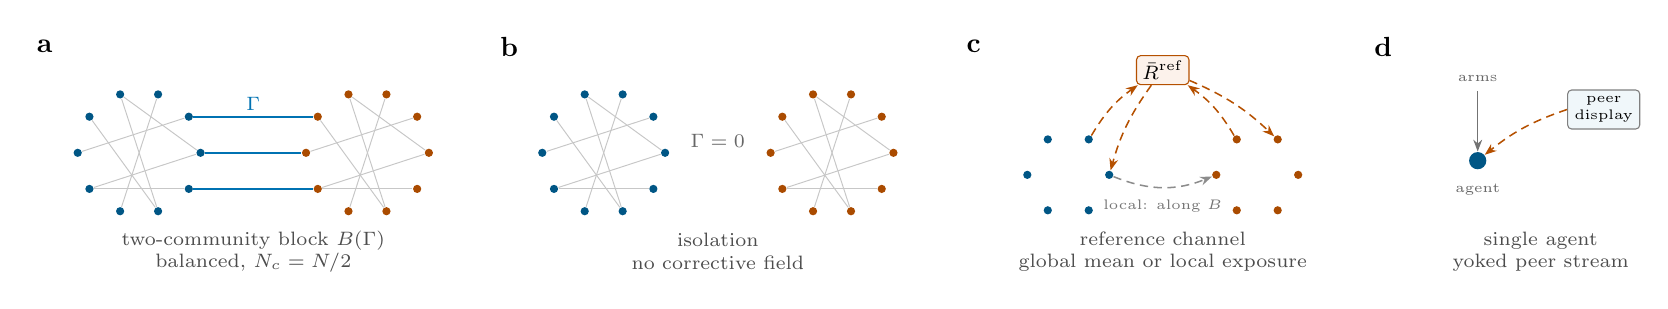
\begin{tikzpicture}[font=\scriptsize,
  agent/.style={circle, fill=black!50, inner sep=1.05pt},
  aA/.style={agent, fill=blu!75!black}, aB/.style={agent, fill=verm!80!black},
  wedge/.style={black!22, line width=.35pt},
  xedge/.style={blu, line width=.75pt},
  refedge/.style={verm!85!black, densely dashed, line width=.55pt, -{Stealth[length=1.5mm]}},
  blab/.style={font=\scriptsize, align=center, text=black!70}]
% ---------- (a) two-community block ----------
\begin{scope}
\node[font=\bfseries] at (-1.2,1.35) {a};
\foreach \i in {0,...,9} \node[aA] (A\i) at ({0.78*cos(36*\i)},{0.78*sin(36*\i)}) {};
\foreach \i in {0,...,9} \node[aB] (B\i) at ({2.9+0.78*cos(36*\i)},{0.78*sin(36*\i)}) {};
\foreach \i/\j in {0/3,1/5,2/7,4/8,6/9,0/6,3/8} {\draw[wedge] (A\i)--(A\j); \draw[wedge] (B\i)--(B\j);}
\draw[xedge] (A0) -- (B5); \draw[xedge] (A1) -- (B4); \draw[xedge] (A9) -- (B6);
\node[text=blu, font=\scriptsize\bfseries] at (1.45,0.62) {$\Gamma$};
\node[blab] at (1.45,-1.25) {two-community block $B(\Gamma)$\\ balanced, $N_c=N/2$};
\end{scope}
% ---------- (b) isolation ----------
\begin{scope}[shift={(5.9,0)}]
\node[font=\bfseries] at (-1.2,1.35) {b};
\foreach \i in {0,...,9} \node[aA] (C\i) at ({0.78*cos(36*\i)},{0.78*sin(36*\i)}) {};
\foreach \i in {0,...,9} \node[aB] (D\i) at ({2.9+0.78*cos(36*\i)},{0.78*sin(36*\i)}) {};
\foreach \i/\j in {0/3,1/5,2/7,4/8,6/9,0/6,3/8} {\draw[wedge] (C\i)--(C\j); \draw[wedge] (D\i)--(D\j);}
\node[text=black!60, font=\scriptsize\bfseries] at (1.45,0.15) {$\Gamma=0$};
\node[blab] at (1.45,-1.25) {isolation\\ no corrective field};
\end{scope}
% ---------- (c) reference channels ----------
\begin{scope}[shift={(11.8,0)}]
\node[font=\bfseries] at (-1.2,1.35) {c};
\foreach \i in {0,...,5} \node[aA] (E\i) at ({0.52*cos(60*\i)},{0.52*sin(60*\i)-0.28}) {};
\foreach \i in {0,...,5} \node[aB] (F\i) at ({2.4+0.52*cos(60*\i)},{0.52*sin(60*\i)-0.28}) {};
\node[draw=verm!85!black, fill=verm!8, rounded corners=1.5pt, inner sep=2pt,
      font=\scriptsize] (RR) at (1.2,1.05) {$\bar R^{\mathrm{ref}}$};
\draw[refedge] (E1) to[bend left=12] (RR);
\draw[refedge] (F2) to[bend right=12] (RR);
\draw[refedge] (RR) to[bend right=10] (E0);
\draw[refedge] (RR) to[bend left=10] (F1);
\draw[refedge, black!45] (E0) to[bend right=22] node[below=1pt, font=\tiny, black!55]{local: along $B$} (F3);
\node[blab] at (1.2,-1.25) {reference channel\\ global mean or local exposure};
\end{scope}
% ---------- (d) single agent + peer display ----------
\begin{scope}[shift={(16.6,0)}]
\node[font=\bfseries] at (-0.8,1.35) {d};
\node[aA, inner sep=2.2pt] (ag) at (0.4,-0.1) {};
\node[below=1.5pt of ag, font=\tiny, black!60] {agent};
\node[draw=black!50, fill=blu!6, rounded corners=1.5pt, inner sep=2.5pt,
      font=\tiny, align=center] (scr) at (2.0,0.55) {peer\\ display};
\draw[refedge] (scr.west) to[bend right=10] (ag);
\draw[-{Stealth[length=1.5mm]}, black!55, line width=.55pt] (0.4,0.78) node[above, font=\tiny, black!60]{arms} -- (ag);
\node[blab] at (1.2,-1.25) {single agent\\ yoked peer stream};
\end{scope}
\end{tikzpicture}}%
\caption{\textbf{Network configurations tested.} \textbf{a}, The balanced two-community
block with permeability $\Gamma$ carries the confirmatory experiment and the dense
maps. \textbf{b}, Isolation ($\Gamma=0$) is the boundary column of those maps and,
with the local reference, the credulous-error cell. \textbf{c}, The two reference
channels of the aspiration update: population mean (global visibility, vermilion) or
exposure-weighted neighbour mean (local, grey). \textbf{d}, The single-agent
configuration behind the analytical checks and the prediction generator (yoked peer
stream in place of a community).}
\label{fig:nets}
\end{figure}

\subsection{Collective failure becomes self-defending: a confirmatory experiment}

We embed the agent in a two-community network in which confidence-weighted choices circulate (permeability $\Gamma$; Fig.~\ref{fig:nets}a and Methods) and give one community an early lead on the inferior arm. At neutral entitlement ($A_0=0.5$) the gate never defeats correction: in frozen baseline experiments, populations correct early lock-ins whether the gate is on or off ($P(\text{defensive wrong})=0.000$, Wilson 95\%~CI $[0,0.019]$, $R=200$ CRN-paired populations), because resignation operates at population scale too. The race condition says where a trap must sit: entitlement above experience, adaptation slower than $\rho_c$, and transmission strong enough that the credibility field holds the wrong action in place while the gate closes.

A fresh-seed confirmatory experiment at the cell fixed in advance by that arithmetic ($A_0=0.8$, $\lambda=0.7$, $\rho=0.002$, $R=300$ runs) passed both pre-stated criteria. Defensive wrong consensus---the losing community locks onto the inferior action with collapsed legitimacy---occurred with probability $0.843$ at the 600-trial horizon (253 of 300 runs; Wilson 95\%~CI $[0.798,0.880]$; criterion $\ge0.5$), and switching the gate off under common random numbers restored $+0.834$ $[0.792,0.872]$ of optimal-choice mass (criterion $\ge0.5$; Fig.~\ref{fig:abm}). An independent reimplementation reproduced the cell (Methods). Entry rides on the initial condition---$A_0=0.8$ stands for entitlement built during remembered affluence---while maintenance is endogenous, through anchoring to the visible winners: delegitimation in this model requires remembered affluence or visible unequal success---never failure alone.

\begin{figure}[t]
\centering
\includegraphics[width=\textwidth]{fig_abm.pdf}
\caption{\textbf{Defensive wrong consensus with fully endogenous entitlement.} \textbf{a}, One trapped run: per-agent legitimacy for all 200 agents; the losing community's gates close within $\sim$100 trials and stay closed, the winning community's dip and recover. \textbf{b}, Path dependence: the losing community's optimal-choice mass over time, 60 gate-on runs (vermilion; most freeze, a minority escape) against 60 gate-off runs (grey; all correct). \textbf{c}, The confirmatory contrast ($R=300$, fresh seeds, common random numbers): terminal optimal mass, gate on versus off; bracket, the paired restore effect with bootstrap 95\% interval. Both pre-stated criteria passed.}
\label{fig:abm}
\end{figure}

\subsection{A sharp, bistable regime boundary in entitlement and transmission}

Dense maps show that the trap occupies a sharply bounded region of the (entitlement, transmission) plane, with the designed validation cell inside it near the front: the probability of defensive wrong consensus rises from 0 to 1 across a narrow band---mean optimal mass falls from $\approx1$ to $\approx0$ over $\Delta A_0\approx0.1$ at $\lambda=0.75$---with the across-run variance peaking exactly there (26$\times$26 cells, 40 runs each; Fig.~\ref{fig:pt1}). The front is bistability, not criticality: terminal outcomes inside it are strictly bimodal (Supplementary Fig.~5), the mean-field dynamics are bistable (Fig.~\ref{fig:flow}), and the front narrows as $N^{-1/2}$ toward the deterministic basin boundary, extrapolating to within $0.03$ of it (Supplementary Section~S12). Near the boundary, early luck selects the regime: path dependence is constitutive of the mechanism.

\begin{figure}[t]
\centering
\includegraphics[width=\textwidth]{fig_pt1.pdf}
\caption{\textbf{The trap is a sharply bounded region.} \textbf{a}, Probability of defensive wrong consensus at the 600-trial horizon over the (entitlement, transmission) plane ($26\times26$ cells, 40 runs each); star, the confirmatory cell; white contour, the empirical $P=0.5$ front; dashed curve, the deterministic basin boundary (Supplementary Section~S5). \textbf{b}, Order-parameter cuts at three transmission strengths (bands, $\pm2$~s.e.m.\ over 60 runs). \textbf{c}, The across-run variance peaks exactly where the order parameter falls---bimodal regime selection, as in Fig.~\ref{fig:abm}b.}
\label{fig:pt1}
\end{figure}

\subsection{Persistence requires entitlement rigidity, and comparison alone cannot save a trap}

A second dense map, over the adaptation rate $\rho$ and the anchoring weight $\chi$, delivers the central insight of the collective analysis: \textbf{persistent collapse is a slow-aspiration phenomenon; social comparison modulates it only inside the slow-adaptation band.} Collapse that persists occupies a band $\rho\lesssim4\times10^{-3}$ almost flat in $\chi$, with the mean-field $\rho_c$ just above the empirical boundary (Fig.~\ref{fig:pt2}a): once behaviour corrects, the population's outcomes---and with them the reference---rise together, so comparison cannot hold aspiration above what experience delivers (Supplementary Section~S4). For empirical work, this relocates the key individual difference from comparison orientation to aspiration rigidity. Persistence is also explicitly horizon-indexed: the empirical boundary falls roughly as $1/T$, because $\rho_c$ governs \emph{absorption}---whether the gate reaches the floor before aspiration adapts---while escape afterwards runs on the aspiration clock $\sim\rho^{-1}$ (Supplementary Section~S12); collapse is a dwell-time phenomenon, not an absorbing phase at infinite time, and dwell times fall sigmoidally around $\rho_c$ (Fig.~\ref{fig:pt2}b). Figure~\ref{fig:race} shows the race itself: one parameter on either side of $\rho_c$ separates a frozen wrong consensus from correction followed by repair.

\begin{figure}[t]
\centering
\includegraphics[width=.9\textwidth]{fig_pt2.pdf}
\caption{\textbf{Persistence is a slow-aspiration phenomenon.} \textbf{a}, Probability that collapse persists to the end of the run over the (anchoring, adaptation-rate) plane at the trap cell ($26\times26$ cells, 40 runs each); dashed line, the closed-form $\rho_c$. The boundary is nearly flat in $\chi$: no level of comparison sustains collapse once aspiration adapts faster than $\approx\rho_c$, because correction lifts the reference together with outcomes. \textbf{b}, Dwell time of collapsed legitimacy against $\rho$ at three anchoring levels (bands, $\pm2$~s.e.m.).}
\label{fig:pt2}
\end{figure}

\begin{figure}[t]
\centering
\includegraphics[width=.92\textwidth]{fig_race.pdf}
\caption{\textbf{The race between collapse and adaptation, watched in time.} Single runs at the confirmatory cell; the trapped panel shows the modal fate ($84\%$ of runs; seed rule and unselected draws: Methods and Supplementary Fig.~7). \textbf{a}, $\rho=0.002<\rho_c$: legitimacy (vermilion) hits the floor within $\sim$100 trials while aspiration (blue, dashed) has barely moved; the optimal mass (ink) freezes---defensive wrong consensus. \textbf{b}, $\rho=0.02>\rho_c$: fast adaptation keeps the gate ajar, behaviour corrects, and legitimacy repairs because post-correction outcomes exceed what aspiration demands. One parameter separates the panels.}
\label{fig:race}
\end{figure}

\subsection{One mechanism, four regimes}

The model generates all four combinations of being right and believing the game fair (Fig.~\ref{fig:mech}b), each in a predictable region. Fast adaptation or low entitlement yields \emph{legitimate consensus}. Slow adaptation and high entitlement yield \emph{defensive wrong consensus} under strong transmission (Fig.~\ref{fig:abm}) but \emph{correct-but-illegitimate} consensus under weak transmission: behaviour corrects ($m_2=0.999$) while legitimacy stays collapsed ($\bar L_2=0.06$). And a fully isolated community locked onto the inferior arm by its own credibility field exhibits \emph{credulous error}: aspiration adapts to the arm's poverty, discomfort stays within tolerance, and the rule retains legitimacy ($m_2=0.001$, $\bar L_2=0.74$)---wrong and content. Collective error and collective grievance are distinct failures with distinct cures, and a dense map over entitlement and permeability realizes all four regimes in a single plane (Fig.~\ref{fig:regmap}).

\begin{figure}[t]
\centering
\includegraphics[width=.9\textwidth]{fig_regimes_map.pdf}
\caption{\textbf{The four regimes realized in one plane.} Modal regime over the (entitlement, permeability) plane at strong transmission ($26\times26$ cells, 40 runs each; classification frozen before execution). All four corners of Fig.~\ref{fig:mech}b appear. Saturation shows the modal regime's frequency (paler = more mixed), so the desaturated seams are the boundaries where identical parameters split between runs; dashed and dotted curves, the deterministic behaviour and legitimacy seams (Supplementary Section~S5).}
\label{fig:regmap}
\end{figure}

Figure~\ref{fig:flow} gives the four regimes their dynamical anatomy: the mean-field flow of aspiration and legitimacy at a representative cell of each regime. Three of the four are genuine attractors. Correct-but-illegitimate is not a fixed point at all but a metastable channel---the dynamical reading of the slow $1/\rho$ recovery clock---which is why the amber region of Fig.~\ref{fig:regmap} is transient in principle yet long-lived at the horizons that matter. The three failures also fail \emph{differently} as information aggregation---at supply, at uptake, and split between layers---a classification the Discussion develops.

\begin{figure}[t]
\centering
\includegraphics[width=.88\textwidth]{fig_flow.pdf}
\caption{\textbf{Dynamical anatomy of the four regimes.} Integral curves of the closed-form mean-field map at four theory-pinned cells (no simulation). Colour gives a trajectory's destination (blue, repair; vermilion, absorption; amber, metastable transit); the grey band is the attracting slow manifold; dashed and dotted verticals, the gate threshold $\Astar(\mu)$ and the aspiration rest point $A_\infty$; the key beneath the panels names every encoding. \textbf{a}, Legitimate consensus: every flow reaches $(A_\infty,1)$. \textbf{b}, Credulous error: the same geometry on the inferior arm---wrong and content is absorbing. \textbf{c}, Defensive wrong consensus: every flow absorbed at $(A_\infty,0)$ while the reference stays high. \textbf{d}, Correct-but-illegitimate is not a fixed point: an amber transit of order $1/\rho$, then repair. Stability: Supplementary Propositions S4.1--S4.3.}
\label{fig:flow}
\end{figure}


\subsection{Transparency heals rational distrust, not grievance}

Is dissonant delegitimation just rational suspicion about the rule? We compared the gate against two Bayesian rival classes (Methods): a \emph{global} class entertaining a rigged-rule hypothesis---both arms pay the inferior rate, for everyone---and a \emph{group-contingent} class whose hypothesis asserts nothing about others' payoffs (the natural form of a grievance about \emph{us}), so visible success elsewhere carries no likelihood either way. The first surprise is who gets trapped. Under isolation at neutral entitlement it is the \emph{Bayesian}: when the whole community earns the rigged-level payoff the hypothesis is self-confirming---the posterior correctly concludes ``rigged'' and learning shuts down---while the dissonance agent rescues itself through resignation.\footnote{Self-confirmation here is an identity, not an artefact of the update rule: the expected log-likelihood-ratio increment equals $\mathrm{KL}(\mathrm{Bern}(\mu_2)\,\|\,\mathrm{Bern}(\mu_{\mathrm{rig}}))-\mathrm{KL}(\mathrm{Bern}(\mu_2)\,\|\,\mathrm{Bern}(\hat\mu))$, which at a wrong consensus ($\mu_2=\mu_{\mathrm{rig}}$) is $-\mathrm{KL}\le0$ for every fair-model estimate $\hat\mu$ (Supplementary Section~S8).} Individual traps of this kind are known in misspecified-learning theory\cite{HeidhuesKoszegiStrack2018,EspondaPouzo2016}; the comparative statement and its network dependence appear to be new.

Transparency then separates the accounts. Across permeability at the trap cell, behaviour corrects for all three agent types once the corrective field dominates ($\Gamma\gtrsim0.15$; Fig.~\ref{fig:trans}a,b), and both rational classes recover trust at evidence speed: the global rival because visible success elsewhere is exactly the evidence that defeats its hypothesis (trust recovers to $1.0$), the group-contingent rival because its still-open prior lets the social field correct behaviour and its \emph{own} improving outcomes then defeat the hypothesis---so the objection that our rival was too coarse strengthens the dissociation rather than weakening it. The dissonance agent is different in kind: its legitimacy does not follow its behaviour, staying collapsed indefinitely at a knife-edge parameter set and otherwise recovering only on the slow $1/\rho$ clock, as aspiration adapts below $\Astar$. The robust dissociation is \emph{timescale separation}: trust recovers at the speed of evidence under rational attribution, but at the speed of aspiration adaptation under dissonance---a population that acts correctly and still believes, for a long time, that the game is rigged.

Direct perturbation locates the trap's scope conditions (Methods; Supplementary Fig.~6). It survives unweighted action frequencies, the retrospective channel off ($\eta=0$), or both ($P_{\mathrm{dw}}=1.00$; 60 runs each), and its size dependence follows the finite-size law ($P_{\mathrm{dw}}=0.63/0.93$ at 60/140 losing agents, against $0.843$ at 100). Two perturbations dissolve it, and both are informative: heterogeneous permeability ($\Gamma_i\in\{0,0.2\}$, mean preserved) corrects every run---the exposed half corrects first and re-transmits through the conformity channel, which the gate does not filter, so the boundary is governed by the most exposed fraction---and payoff-biased imitation, whose success-weighted copying amplifies lucky deviants where confidence-weighted copying amplifies the confident majority. Defensive wrong consensus is therefore a pathology of conformist, confidence-weighted transmission under uniformly weak outside contact---where cultural evolution has long located maladaptive traditions\cite{BoydRicherson1985}---and both conditions are testable predictions; in both dissolving cases behaviour corrects while legitimacy sits near $0.4$, so the timescale dissociation survives the loss of the trap. These scope conditions become quantitative at scale.

\subsection{The window: from two communities to arbitrarily many}

Nothing in the theory is special to two communities: the general architecture couples $M$ communities of any sizes through a row-stochastic exposure matrix $W$, with the two-community $B(\Gamma)$ its smallest case.\footnote{Block-uniform exposure keeps the community-level field exact at every $M$ and any size profile, so the general engine aggregates without approximation; the validation gate and all records are in the repository.} The number of communities is irrelevant in a precise sense: over a fixed horizon, a community's fate depends only on its depth-limited exposure neighbourhood, so the per-community law is unchanged once that neighbourhood stabilizes and converges as $M\to\infty$ along locally convergent meta-networks (Supplementary Section~S13.7). What a battery can test is therefore not scale but structure. We ran one, frozen in advance, across $M\in\{2,10,100,1000,10{,}000\}$ at fixed population ($N=10{,}000$; $N=100{,}000$ at the largest $M$), with ring, Watts--Strogatz, preferential-attachment and broadcast meta-networks, clustered and scattered losing halves, and unequal community sizes (Methods; Supplementary Section~S13).

A two-level law organizes everything (Fig.~\ref{fig:window}a,b). The first level is a losing community's \emph{structural} cross-exposure to initially-corrected communities, $x_c=\sum_{d\,\mathrm{correct\,at}\,t=0}W_{cd}$---fixed by the graph and the initial assignment, nothing about it an outcome. Across 266,400 community outcomes, exposure locates two edges: below $x\approx0.075$, defensive wrong consensus at the 600-trial horizon is near-certain in every geometry; above $x\approx0.1125$, escape is near-certain in every architecture tested. The second level, community size, decides between the edges: conditional on size, exposure acts almost as a step---communities of a hundred or more trap throughout the window; ten-agent communities seed escapes that cascade, each corrected fellow loser adding exposure beyond $x$. Hence the ladder of Fig.~\ref{fig:window}a is flat in $M$ at fixed size: scale does nothing that size does not---the finite-$M$ face of the limit statement above.\footnote{Pooled over the battery, terminal class is predicted from $x$ alone with AUC $0.92$; adding community size raises it to $0.96$, and geometry dummies add almost nothing further ($0.97$): geometry acts through the exposure and size profiles it induces, not on its own. Meta-degree is irrelevant \emph{by construction}: the exposure budget is fixed, so degree can move only the composition of exposure, and on preferential-attachment graphs trap probability is accordingly flat in degree ($0.62$--$0.71$).}

The window runs on two clocks. The gate reopens---entitlement falls below $\Astar$---at the closed-form time $t^{*}(x)=\rho^{-1}\ln\!\bigl[(A_0-A^{\mathrm{eq}})/(\Astar-A^{\mathrm{eq}})\bigr]$ with $A^{\mathrm{eq}}=\mu_2+\chi x(\mu_1-\mu_2)$: $896$ to $980$ trials at every realized exposure, which is why every trapped community is still trapped at the 600-trial horizon. But a reopened gate is not a healed one: repair fights the continuing failure stream, so legitimacy is restored only at $t^{**}\approx1.4$--$1.5\times t^{*}$---confirmed out of sample: communities fully trapped at $1{,}100$ trials resolve by $1{,}600$, into a credulous majority with correction spreading in from the cluster's edge (Fig.~\ref{fig:window}d). Grievance outlives its own gate: losing the entitlement is faster than forgiving the game. Permanence would require the equilibrium-reference condition $\chi\,x_c\,(\mu_1-\mu_2)>\Astar(\mu_2)-\mu_2$---at the frozen parameters $x_c>5/6$, unreachable in every battery---so every trap is horizon-indexed. And cross-exposure \emph{lengthens} grievance ($dt^{*}/dx>0$): visible winners keep entitlement alive even as they fail to flip behaviour.

Two consequences deserve notice. First, a common broadcast corrects exactly when its weight times the winners' share of the field crosses the escape edge (confirmed out of sample): what looked like correction at scale is a community-size effect---at fixed size the broadcast traps at every $M$ we test, and the correction at $M=1000$ was a ten-agent cascade amplified by the common field, which then leaves $45\%$ of losing communities corrected-but-illegitimate (Fig.~\ref{fig:window}c). Second, the window is the echo-chamber condition stated in exposure units: enough contact to sustain the grievance, not enough to flip the behaviour. One methodological note: these laws were first assembled from a battery whose own pre-stated predictions they superseded, so we re-froze them as predictions and ran a second, preregistered battery---the two-level law, the $M$-invariance at fixed size, and both clocks held out of sample, and the two places the first battery's phrasing failed are corrected in Supplementary Section~S13.6.

\begin{figure}[t]
\centering
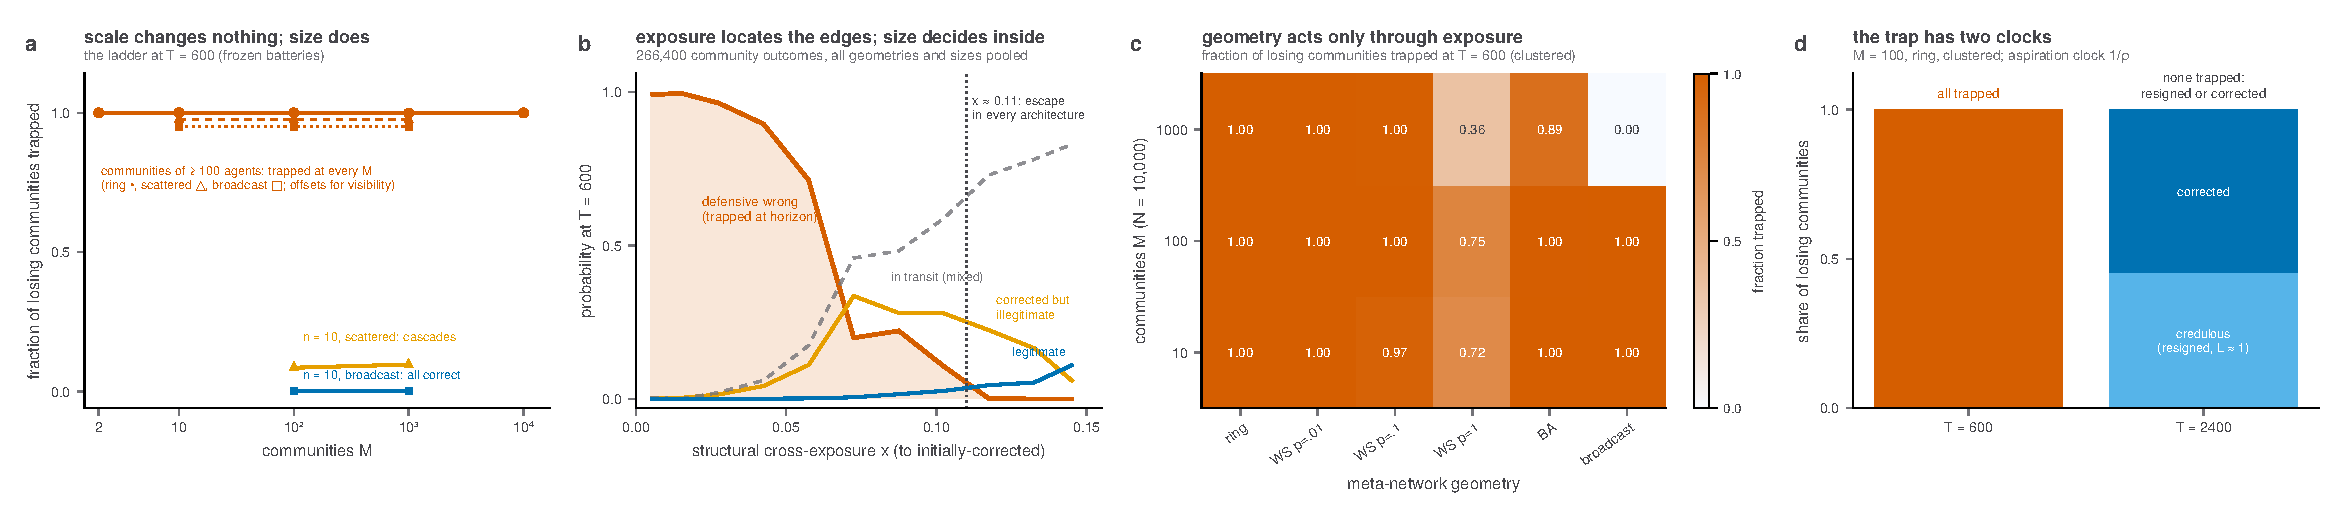
\includegraphics[width=\textwidth]{fig_window.pdf}
\caption{\textbf{The exposure window governs the trap at every scale.} Frozen $M$-community battery ($M=2$--$10{,}000$; ring, Watts--Strogatz, preferential-attachment and broadcast meta-networks; clustered and scattered losing halves; Methods and Supplementary Section~S13). \textbf{a}, The ladder, $M=2$ to $10{,}000$: trap fraction is flat in $M$ at fixed community size---communities of $\ge100$ agents trap under every geometry, broadcast included, while ten-agent communities escape by cascade---so scale does nothing that size does not. \textbf{b}, Probability of each terminal class at $T=600$ against structural cross-exposure $x$ to initially-corrected communities, pooled over all geometries and sizes. The graded middle is composition: conditional on community size, $x$ is close to a step, with escape near-certain above $x\approx0.11$ in every architecture (Supplementary Section~S13). \textbf{c}, Fraction of losing communities trapped (clustered placement) by geometry and $M$: geometry acts through the exposure and size profiles it induces. \textbf{d}, The two clocks at $M=100$ (ring, clustered): every losing community trapped at $T=600$, none at $T=2400$---$45\%$ resign into credulous error, the rest correct; resolution sits near $t^{**}\approx1.4\times t^{*}$ (Supplementary Section~S13).}
\label{fig:window}
\end{figure}

Two single-agent signatures discriminate dissonant delegitimation from rational rule-suspicion. First, a \emph{recovery threshold}: after collapse, reopening time diverges as restored outcome quality approaches the resignation boundary ($3\times10^4$ trials at $\mu_{\mathrm{good}}=0.5$ versus $10^2$ at $0.9$), while the Bayesian recovers smoothly at any quality (Fig.~\ref{fig:trans}c)---``too little, too late'' is a dissonance-specific threshold. Second, \emph{entitlement scaling}: collapse time falls steeply in initial entitlement under identical outcome streams, whereas fixed-hypothesis Bayesian updating is invariant to entitlement framing by construction (Fig.~\ref{fig:trans}d). A third---graded downward steps versus repair capped at $\nu_R$---requires rating-type data. Against an \emph{unconstrained} Bayesian whose priors respond to framing, the static signatures lose force; the dynamic ones (threshold, timescale separation, increment asymmetry) survive that identification wall, and we state this boundary rather than hide it.

\begin{figure}[t]
\centering
\includegraphics[width=.88\textwidth]{fig_transparency.pdf}
\caption{\textbf{Transparency dissociates dissonance from rational rule-suspicion.} \textbf{a},\,\textbf{b}, Permeability sweeps at the trap cell (26 values, 60 runs each; bands, $\pm2$~s.e.m.): optimal mass (\textbf{a}) and the trust variable (\textbf{b}) for the dissonance agent (vermilion), the global rigged-rule Bayesian (blue) and the group-contingent Bayesian (sky, dash-dotted). Behaviour corrects for all three; both rational classes recover trust at evidence speed, dissonant legitimacy only on the slow $1/\rho$ clock (dashed). \textbf{c}, Reopening time against restored quality: the dissonance agent diverges at the resignation boundary; the Bayesian recovers smoothly. \textbf{d}, Collapse time scales with initial entitlement; fixed-hypothesis Bayesian collapse is entitlement-invariant.}
\label{fig:trans}
\end{figure}

\subsection{What can be measured}

The mechanism's boundaries are themselves results: connectivity has no interior welfare minimum on the tested domain (the comparison channel's damage appears only in legitimacy, never in earnings), and the signatures above are the survivors of a frozen adversarial screen whose rejected candidates and counterexamples are preserved in the Supplement and repository. A synthetic-recovery programme across three generations of task designs and estimators (Methods) then fixes the scope of any empirical test. The gate's loss, repair and tolerance parameters are not individually recoverable from choices plus periodic legitimacy ratings at realistic scale---the likelihood has structural ridges\footnote{Two ridge systems: $(\nu_F,\tau^F)$ trade off along the collapse slope, and $(\nu_R,\rho,\chi)$ through the latent aspiration path; the likelihood geometry, the full recovery screens and the confusion matrices are in Supplementary Section~S9.}, and per-interval legitimacy increments sit below plausible rating noise. Eliciting the \emph{aspiration itself} breaks the latent-aspiration ridges exactly as the theory predicts: individual recovery of the adaptation rate $\rho$ jumps from $r=0.33$ to $r=0.91$ (maximum likelihood, $L$ alone versus $L{+}A$; the MAP contrast is $0.53$ to $0.91$; Extended Data Fig.~1). Group means of the collapse-side parameters are nearly unbiased at modest samples ($\nu_F$, $+1.5\%$; $\tau^F$, $+2.4\%$), while the repair rate is not ($-30\%$). And likelihood-based model comparison cannot separate the gate from inequity-in-utility accounts of the kind fitted to recent inequity-learning data\cite{HamJenkins2025}: at the best design-estimator cell, only 11 of 20 dissonance-generated subjects are recovered as dissonant and 9 are claimed by the aspiration-in-utility model---a confusion diagonal of $0.55$ (Supplementary Section~S9). The gate-versus-utility question must be decided by the dynamic signatures, not by model selection---a constraint we regard as a deliverable, in the spirit of computational-modelling good practice\cite{WilsonCollins2019}, fixed before any participant is recruited.

\subsection{The model commits to testable predictions}

A mechanism earns the name only if it constrains an experiment, so we close by committing the model to predictions in the exact geometry of the preregistration-ready task: a three-phase bandit (rich, deprived, restored) with a yoked no-deception peer-earnings display---reference regime HIGH (visibly successful peer) or LOW (peer matched to own outcomes)---and fairness and entitlement sliders every five trials (Fig.~\ref{fig:pred}a). Everything in Fig.~\ref{fig:pred}b--e is model output at the frozen agent specification, generated before any participant exists; none of it requires model fitting to test.

The simulations answer every question that does not require a human, so the experiment is the smallest humans-by-treatments grid that confirms the central prediction and identifies what no simulation can: whether the gate exists in people, and the human distribution of aspiration rigidity. It tests \textbf{two hypotheses in series} (gatekeeping, so the family-wise error stays at $\alpha=0.005$ with no splitting). \emph{H1a, reference-dependent delegitimation}: holding own outcomes fixed, the deprivation-phase fall in rated fairness is larger under a HIGH than a LOW peer reference---a one-sided rank test on the P1$\to$P2 drop, measured distribution-free as $\theta=P(\mathrm{drop}_{\mathrm{HIGH}}>\mathrm{drop}_{\mathrm{LOW}})$, $N=320$ per reference arm pooled across restoration arms, powered $\ge0.90$ at the design basis $\theta=0.592$ worst case over a six-shape battery (Methods). \emph{H1b, tested only if H1a rejects---the gate itself}: under moderate restoration, choice accuracy recovers above a pre-stated floor while rated fairness stays inside an equivalence band excluding the utility rival's predicted recovery, the band and its power fixed from pilot rating noise before registration. Within each reference arm, moderate and full restoration are allocated 2:1---the mass sits where H1b lives; the full arm is the positive control. The within-subject entitlement slider yields each participant's aspiration rigidity: the one quantity the simulations cannot supply, and the instrument that carries the lab into the field. Table~\ref{tab:pred} collects the predictions against their nearest rivals.

\begin{table}[t]
\small
\caption{\textbf{What the experiment will show.} Serial gatekeeping holds the family-wise error at $\alpha=0.005$; H1b is tested only if H1a rejects. Secondaries are preregistered as discriminating, never confirmatory.}
\label{tab:pred}
\begin{tabular}{@{}p{0.15\textwidth}p{0.31\textwidth}p{0.27\textwidth}p{0.18\textwidth}@{}}
\hline
 & Gate predicts & Closest rival predicts & Test \\
\hline
\textbf{H1a} (confirmatory) & P2 fairness drop larger under HIGH than LOW reference at identical own outcomes & inequity-in-utility: same sign at roughly half size; global-rig Bayesian: null or reversed & one-sided rank test (WMW); $N{=}320$/arm; power $\ge0.90$ at $\theta{=}.592$, worst case over a six-shape battery \\
\textbf{H1b} (co-confirmatory, gatekept) & under moderate restoration, choice accuracy recovers while rated fairness stays flat & utility rival recovers ratings alongside behaviour & TOST band $\pm\delta_{\mathrm{eq}}$ from pilot noise \\
H2 (secondary) & behavioural recovery at evidence speed; trust lags on the aspiration clock & every instantiated Bayesian recovers both at evidence speed & condition $\times$ measure midpoint lag \\
H3 (secondary) & reopening needs restored quality above a threshold (``too little, too late'') & graded recovery at any restored quality & Reference $\times$ Restoration interaction \\
H4 (secondary) & rating decrements scale with entitlement shortfall; increments capped & symmetric in surprise & mixed-effects increment asymmetry \\
Framing probe & the drop persists under fixed-rate group-contingent framing: grievance, not inference & group-contingent Bayesian banks P1 evidence---no drop & secondary contrast \\
\hline
\end{tabular}
\end{table}

Figure~\ref{fig:pred}b--e walks the predictions past their rivals. The confirmatory target (panel~b) is singular by design: under identical own outcomes, predicted fairness falls substantially further under HIGH than under LOW reference, because the visible peer holds the entitlement benchmark above what experience delivers. The rivals separate in panel~c: the global rigged-rule Bayesian is \emph{rescued} by the successful peer and collapses under LOW; the group-contingent Bayesian banks the rich first phase and predicts essentially no drop; the aspiration-in-utility rival mimics a reference-ordered drop at roughly half size ($19$ against $45$ rating points under HIGH). The drop alone therefore cannot decide gate versus utility; the restoration phase can (panel~d): choice accuracy recovers within tens of trials while gated fairness crawls, flatlining under moderate restoration ($43$ and $14$), whereas the utility rival recovers fully at either level ($97$ under full, $89$ under moderate)---``too little, too late'' as a measurable flatline. Panel~e shows the increment asymmetry: decrements graded in the elicited shortfall, increments capped near the repair rate, where the utility rival moves symmetrically. Against richer reference-dependent-prior Bayesians, discrimination falls, as preregistered, to these dynamic signatures. The design is not powered at the edge of its own theory.\footnote{Model-implied effect sizes span $d=1.8$--$6.6$ with power above $0.999$---upper bounds by construction (Supplementary Section~S12). The binding arithmetic is distribution-free: Monte Carlo rank-test power over six non-normal shapes incl.\ an exclusion-selection cell gives $N^{*}(0.90)=320$/arm at $\theta=0.592$ ($\approx d=0.33$ under normality); mean-shift tests lose up to half their power under the skewed shapes, hence the rank test is primary. At the $\theta=0.570$ floor, power is $0.65$--$0.72$, reported rather than claimed; H1b's band and power come from pilot noise before registration.} The full hypothesis set, exclusion rules, sample sizes and decision rules---including which outcomes would refute the gate---are fixed in the accompanying preregistration documents.

\begin{figure}[p]
\centering
% ---- panel a: task protocol strip (TikZ) ----
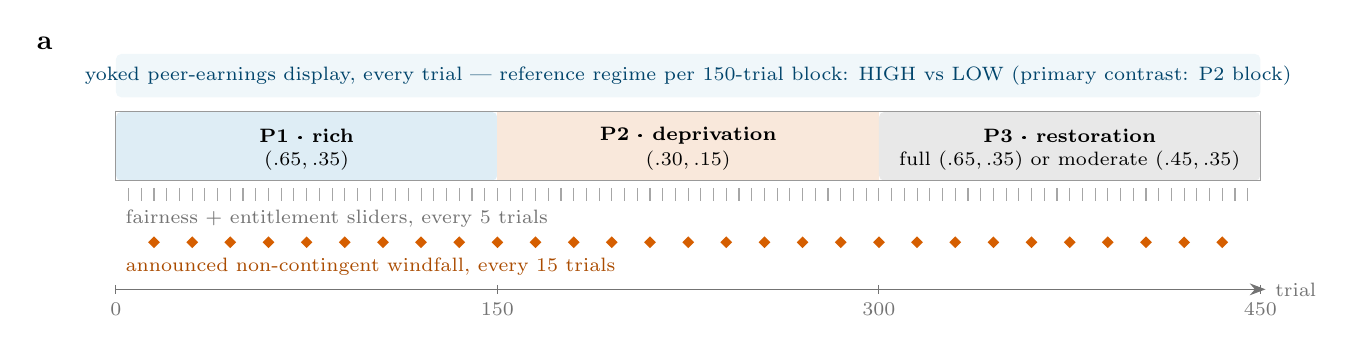
\begin{tikzpicture}[font=\small, xscale=0.0323, yscale=.92]
\node[font=\bfseries] at (-28, 1.9) {a};
% peer display band
\fill[blu!6, rounded corners=2pt] (0,1.15) rectangle (450,1.75);
\node[font=\scriptsize, text=blu!60!black] at (225,1.45)
  {yoked peer-earnings display, every trial --- reference regime per 150-trial block: HIGH vs LOW (primary contrast: P2 block)};
% phase bar
\fill[blu!13, rounded corners=2pt]  (0,0)   rectangle (150,0.95);
\fill[verm!14] (150,0) rectangle (300,0.95);
\fill[black!9, rounded corners=2pt] (300,0) rectangle (450,0.95);
\node[font=\scriptsize\bfseries] at (75,0.62)  {P1 · rich};
\node[font=\scriptsize] at (75,0.28)  {$(.65,.35)$};
\node[font=\scriptsize\bfseries] at (225,0.62) {P2 · deprivation};
\node[font=\scriptsize] at (225,0.28) {$(.30,.15)$};
\node[font=\scriptsize\bfseries] at (375,0.62) {P3 · restoration};
\node[font=\scriptsize] at (375,0.28) {full $(.65,.35)$ or moderate $(.45,.35)$};
\draw[black!40] (0,0) rectangle (450,0.95);
% slider cadence
\foreach \x in {5,10,...,445} \draw[black!35, line width=.4pt] (\x,-0.1) -- (\x,-0.28);
\node[font=\scriptsize, text=black!55, anchor=west] at (0,-0.52) {fairness + entitlement sliders, every 5 trials};
% windfalls
\foreach \x in {15,30,...,435} \node[fill=verm, diamond, inner sep=1.1pt] at (\x,-0.85) {};
\node[font=\scriptsize, text=verm!80!black, anchor=west] at (0,-1.18) {announced non-contingent windfall, every 15 trials};
\draw[-{Stealth[length=2mm]}, black!55] (0,-1.5) -- (452,-1.5) node[right, font=\scriptsize, black!55]{trial};
\foreach \x in {0,150,300,450} \draw[black!55] (\x,-1.44) -- (\x,-1.56) node[below, font=\scriptsize]{\x};
\end{tikzpicture}\\[2.5mm]
\includegraphics[width=.9\textwidth]{fig_pred.pdf}
\caption{\textbf{Model-generated predictions for the preregistered experiment.} All curves are model output, not data (Methods). \textbf{a}, The task: three phases, a yoked no-deception peer display (reference regime HIGH or LOW), two sliders every five trials, announced windfalls. \textbf{b}, The confirmatory target: predicted fairness falls much further in P2 under HIGH than LOW at identical own outcomes (mean and interquartile band, 300 simulated subjects). \textbf{c}, Rivals with the same display: the global rig reverses the ordering (blue); the group-contingent rig predicts no drop (sky, dash-dotted); the aspiration-in-utility rival (amber, dotted) mimics a drop half the gate's size with fast recovery. Presence, direction and size of the reference effect separate the four accounts. \textbf{d}, P3 under HIGH: accuracy (ink) recovers fast; gated fairness (vermilion) crawls, and flatlines under moderate restoration; the utility rival (amber) recovers even there---P3 decides gate versus utility. \textbf{e}, Rating change against elicited shortfall: erosion graded, repair capped near $\nu_R$.}
\label{fig:pred}
\end{figure}

\section{Discussion}

Treating ``learn from the outcome'' and ``question the game'' as margins of one dissonance problem turns two free-standing behavioural postulates into one as-if objective with stated coupling restrictions. The representation has bite: it forces entitlement to be a state variable, and entitlement's dynamics---not the gate itself---govern everything collective. Persistent defensive error requires entitlement held above experience, whether by rigidity, by culture, or by visible unequal success; shared or invisible failure breeds resignation instead of grievance. That is a scope condition the literatures on system justification and relative deprivation have long needed\cite{JostBanajiNosek2004,SmithPettigrew2012}: which pattern appears is predicted by reference-group exposure and aspiration rigidity, not by deprivation itself---a trap entered through entitlement, exited through adaptation, and selected by early stochastic history near the front.

The transparency dissociation is the model's sharpest comparative static, and we state it as a comparative static, since the model prices neither transparency nor welfare. Visibility of others' success is exactly the evidence that heals rational distrust of a rule---and, through the corrective field, it heals behaviour under both accounts---yet it is also exactly the anchor that sustains dissonant grievance on a slow clock after behaviour has healed. Interventions that restore accurate feedback can therefore fix what people do while leaving intact what they believe about the game's fairness. Rational accounts of self-confirming distrust\cite{HeidhuesKoszegiStrack2018,EspondaPouzo2016,FrickIijimaIshii2020,BohrenHauser2021} cannot produce this combination: in that family, distrust is an isolation phenomenon dissolved by visibility; here, grievance is a comparison phenomenon sustained by it. Network epistemology has taught that connectivity's value depends on what it carries\cite{Zollman2007}; we add that its valence depends on whether it carries evidence or reference points, and for which kind of agent.

The same results locate the model within the theory of information aggregation. Classical conditions for crowd wisdom are structural---naive pooling aggregates when no agent retains outsized influence\cite{DeGroot1974,GolubJackson2010}---and classical failures are supply-side: cascades persist because early actions conceal the private signals behind them\cite{Banerjee1992,BikhchandaniHirshleiferWelch1992}. Both accounts fix the weight an agent places on evidence. Making that weight a state variable breaks the link between structure and aggregation quality in the class we study (two-community blocks under conformist transmission; the structural perturbations above mark the class boundary, and degree-heterogeneous graphs beyond the permeability perturbation remain open): a network that satisfies the structural conditions for aggregation still fails to aggregate for the community whose outcomes lag its entitlement, because the weights collapse precisely where corrective information is concentrated. This is a third failure mode for collective wisdom---evidence refused at uptake---distinct from correlated signals and unbalanced influence, and the distinction is exactly Nguyen's\cite{Nguyen2020}: a bubble omits outside voices and is cured by exposure; a chamber discredits them and survives it. Defensive wrong consensus is an echo chamber in this strict sense, built by the gate out of outcome--entitlement gaps rather than homophilous curation\cite{Cinelli2021}---which is why cross-cutting exposure can correct behaviour while leaving distrust intact, the pattern reported when opposing views are injected into field feeds\cite{Bail2018}. Supplying more information, better routed, repairs the first two failures; the third moves only on the entitlement side, through aspiration adaptation and reference-group exposure.

Two of the model's components meet measurement literatures directly. First, learning asymmetries: because the gate makes the effective learning rate $\alpha L_t$ state-dependent, fitting a standard dual-learning-rate model of optimistic reinforcement learning\cite{Lefebvre2017} to gate-generated choices yields an apparent positivity bias that is induced rather than trait-like---in a frozen check on the task geometry, the fitted asymmetry $\log(\alpha^+/\alpha^-)$ shifts by $+0.48$ from the rich to the deprivation phase under a HIGH reference ($+0.33$ under LOW), against at most $+0.11$ with the gate off (Supplementary Section~S12). Where normative accounts derive fixed asymmetries from the environment's reward statistics\cite{CazeVanDerMeer2013}, the gate predicts a moderation by elicited shortfall and reference regime, tested in the choice data at no extra cost. Second, the model's two social quantities have measurement and neural literatures of their own: the credibility field's decisiveness weighting is the confidence weighting that governs advice uptake and trust formation\cite{PescetelliYeung2021,PescetelliHauperichYeung2021}; the slider-elicited reference and entitlement computations are of the kind dorsomedial frontal cortex tracks in social-comparison settings\cite{Wittmann2016,Wittmann2025}; and lesion evidence that ventromedial prefrontal damage selectively disrupts prosocial motivation and learning to reward others\cite{Lockwood2024,Gueguen2025} shows socially contextualized valuation is causally dissociable from its self-referential counterpart---precisely what a legitimacy gate on socially benchmarked outcomes requires. The three-phase task is imaging- and lesion-compatible, a route from algorithm to substrate.

The empirical programme is constrained, deliberately, by our own identifiability results: ratings plus an entitlement elicitation recover individual aspiration rigidity and group-level gate parameters, and the gate-versus-utility question rests on dynamic signatures rather than model selection. The inequity-learning finding\cite{HamJenkins2025} supplies a candidate paradigm; the gate supplies its mechanism; the simulations supply the effect sizes, the moderator, and the honesty constraints. The programme is staged: the preregistered experiment targets one confirmatory prediction---reference-dependent delegitimation---with the discriminating dynamics as preregistered secondaries, and its individual-level output, aspiration rigidity, then anchors a field analysis of the same signatures in social-media data, where reference exposure and legitimacy-laden language are observable and horizon-indexed persistence becomes an object of measurement rather than simulation. The exposure window makes that stage concrete: the field analysis must estimate the distribution of structural cross-exposure $x$ a platform induces, because the theory locates every community's fate on it, and the two clocks convert a measured rigidity distribution into a predicted persistence distribution---a falsifiable quantity rather than a direction. Limitations are stated in Methods; chief among them, the dissonance minimization is myopic, the formal layer certifies algebra only, and the collective results are class-conditional, with the class boundary located but not exhausted by the structural perturbations above.

\section{Methods}

\subsection{Model}
$N$ agents in $M$ communities choose repeatedly between two arms with Bernoulli means $\mu_1>\mu_2$; community coupling is a row-stochastic exposure matrix $W$ over communities, and every confirmatory experiment uses the two-community worked case ($M=2$, equal halves).\footnote{The agent-based model is fully documented under the ODD+D protocol\cite{Muller2013,Grimm2020} in the public repository (\texttt{ODD\_D.md}, \texttt{github.com/TrompetteMarine/CSL3}), together with the frozen-design records, the engine cross-validation and the complete reproducibility protocol; the Methods here state only what is needed to read the results.} There $W=B=\bigl(\begin{smallmatrix}1-\Gamma & \Gamma\\ \Gamma & 1-\Gamma\end{smallmatrix}\bigr)$ with permeability $\Gamma$: an agent's social input weights its own community by $1-\Gamma$ and the other by $\Gamma$. The $M$-community battery builds $W$ from meta-network geometries (Supplementary Section~S13). Agent $i$ holds values $Q_{i,t}(a)\in[0,1]$, legitimacy $L_{i,t}\in[0,1]$, aspiration $A_{i,t}\in[0,1]$. The anticipatory field is the decisiveness-weighted action mass: $\phi_{c,t}(a)=\tfrac1{N_c}\sum_{j\in c}\1\{a_{j,t}=a\}C_{j,t}$, $S_{i,t}(a)=\sum_d B_{c(i)d}\phi_{d,t-1}(a)$; augmented values $V=Q+\lambda S$; choice $\Prob(a{=}1)=\Lambda(2\beta a_{\mathrm{thr}}(V(1)-V(2))/\sigma^2)$, which is the first-passage probability of a symmetric-threshold diffusion with drift $\beta(V(1)-V(2))$, noise $\sigma$ and threshold $a_{\mathrm{thr}}$---we use only this choice-probability reduction and model no response times\footnote{Response-time-level diffusion phenomena are therefore outside the model's claims; in particular, fast errors require starting-point variability, which the reduction neither uses nor implies. The experimental task records response times for exploratory analysis only.}; decisiveness $C=|2\Prob-1|$, a confidence-like weight of the kind that governs human advice uptake\cite{PescetelliYeung2021}. A retrospective channel revises values towards decisiveness-weighted observed outcomes with gain $\eta$, gated like the private channel. All prediction errors and the discomfort $D^F$ use pre-update states; updates are synchronous. The reference outcome $\bar R^{\mathrm{ref}}$ in the aspiration update is the exposure-weighted neighbour mean (``local'') or the population mean (``global visibility''); figures state which. The interaction structures used across all experiments are collected in Fig.~\ref{fig:nets}. Defaults in Table~\ref{tab:params}; $\nu_R/\nu_F=0.25$ places $\Astar$ strictly away from both arm means (an earlier default created a knife-edge $\Astar(0.6)=0.6$, removed before confirmatory work; the knife-edge variant is shown only where stated, for continuity with audited runs).

\begin{table}[H]\centering\small
\caption{Default parameters.}
\label{tab:params}
\begin{tabular}{llp{7.2cm}}
\toprule
Symbol & Default & Role \\
\midrule
$\mu_1,\mu_2$ & $0.6,\,0.4$ & arm means \\
$\lambda$, $\eta$ & $0.5$, $0.2$ & anticipatory / retrospective social weights ($\lambda$ is the text's ``transmission'') \\
$\beta,\sigma,a_{\mathrm{thr}}$ & $6,1,1$ & quantal choice \\
$\alpha$ & $0.2$ & private learning rate \\
$\nu_F$, $\nu_R$ & $0.05$, $0.0125$ & legitimacy loss / repair \\
$\tau^F$; $\phi^-,\phi^+$ & $0.3$; $1,0.25$ & tolerance; discomfort asymmetry \\
$\rho$, $\chi$ & scenario & aspiration adaptation / anchoring \\
$N$; $T$ & $200$; $600$ & agents; trials \\
\bottomrule
\end{tabular}
\end{table}

\subsection{Derivation and analytical results}
Equation~\eqref{eq:updates} follows from $\partial\mathcal D/\partial Q(a_t)=-L(R_t-Q(a_t))$ (gain $\alpha$) and from the frame margin's linearity in $L$ with slope $w_f(X_t-\kappa K_t)$ (gain $\nu$; $\nu_F=\nu w_f$, $\nu_R=\nu w_f\kappa$). If the frame margin also sees the evidence term, the update gains a surprise-erosion term $-\nu\delta^2/2$; the threshold structure survives with shifted constants. Defaults satisfy the windfall-corner restriction $\phi^+\le\tau^F/(1-\tau^F/\phi^-)$ (Supplementary Section~S3), which excludes delegitimation triggered by windfalls above aspiration; outside it the effect is transient and self-extinguishes as aspiration adapts upwards (a 20-run illustration at $\phi^+=0.5$ dips to mean legitimacy $0.70$ around trial 190 and recovers to $0.99$ by the horizon; Supplementary Section~S12). The drift, $\Astar$ (equation~\eqref{eq:astar}), resignation, relative deprivation, and the race condition
\begin{equation*}
\rho_c=\frac{\nu_F(1-\mu_2)\phi^-}{L_0}\Big[(A_0-\Astar)-(\Astar-\mu_2)\ln\tfrac{A_0-\mu_2}{\Astar-\mu_2}\Big]
\end{equation*}
are derived in the generic region ($\phi^-A>\tau^F$, $\phi^+(1-A)\le\tau^F$); the full four-region drift decomposition, proofs, the mean-field reduction of the network model, and the stochastic-approximation connections (including an explicit list of what is \emph{not} proved) are in Supplementary Sections S3--S6, with corner regimes (windfall delegitimation; absolute deprivation) excluded from headline claims by stated parameter restrictions. Relearning after reopening is governed by the contraction $Q'-\mu=(1-\alpha L)(Q-\mu)$. Every proposition was verified numerically on parameter grids before any network experiment.


\subsection{The Bayesian rivals}
The rational comparison agents replace the gate by a posterior over rule validity, with effective learning rate $\alpha\,\pi_t(\mathrm{fair})$ and choice on model-averaged values. The \emph{global} class holds $H_{\mathrm{fair}}$ (arms pay their learnable means) versus $H_{\mathrm{rig}}$ (both arms pay Bernoulli $0.4$ for everyone), updated by likelihood on own outcomes and exposure-weighted observed outcomes. The \emph{group-contingent} class holds the same $H_{\mathrm{rig}}$ about its own payoffs only, so observed others contribute zero log-likelihood by construction; it was added in response to the objection that grievances are typically group-indexed, and its network and task-protocol behaviour are reported in the Results and Supplementary Section~S8. Both are deliberately simple members of the misspecified-learning family\cite{EspondaPouzo2016,HeidhuesKoszegiStrack2018,Bohren2016}; their role is comparative. The self-confirming-trap mechanism---the expected log-likelihood increment is maximized at zero exactly when the community's earnings match the rigged rate---is derived in Supplementary Section S8.

\subsection{Robustness}
Supplementary Section~S12 reports, under frozen designs: the finite-size and horizon scaling behind the bistability and dwell-time readings (with the $N\to\infty$ front extrapolation and the direct absorption test of $\rho_c$); classification-threshold insensitivity; the non-lexicographic variant (the trap survives and strengthens, and the variant's divergence at neutral entitlement makes the lexicographic convention testable); the structural and field-form perturbation battery behind the scope conditions of the Results; a Morris screening over twelve parameters (permeability dominates globally; the microparameters are negligible at this horizon), which contextualizes but does not replace the slice-conditional claims; the induced learning-rate asymmetry check; and the rating-noise sensitivity of the identification study---whose load-bearing conclusion, individual recoverability of $\rho$, holds at double the assumed noise ($r=0.80$ against the $0.7$ gate).

\subsection{Identification study}
Synthetic-recovery programme over three task/estimator generations; final generation: three-phase bandit (baseline, deprivation, restoration; $T=450$), sustained peer-reference display with block-randomized regimes, announced non-contingent bonus trials, legitimacy and aspiration sliders every 5 trials (rating noise $\sigma=0.1$); estimators, maximum likelihood and MAP with deliberately weak priors; model set, the dissonance agent, the Bayesian rival, an associability (Pearce--Hall) learner\cite{PearceHall1980}, and an aspiration-in-utility learner in the class fitted by Ham and Jenkins\cite{HamJenkins2025}; selection by BIC with all models accounting for all observations. Headline outcomes in the text; the likelihood geometry behind the two ridge systems, full screens, group-bias bootstraps and confusion matrices are in Supplementary Section S9 and the bundle.

\subsection{Prediction generation}
The prediction figure (Fig.~\ref{fig:pred}) is generated, not fitted: 300 simulated subjects per condition run the frozen agent specification of Table~\ref{tab:params} (fairness slider $=100L$; entitlement slider $=100A$) through the task---three phases, yoked reference display, sliders every five trials---with the rigidity moderator as an equal slow/fast mix and anchoring $\chi=0.6$. The Bayesian rivals are those of the transparency analysis observing the same display; the aspiration-in-utility rival is ported verbatim from the identification study's utility class, including that class's own rating link, so the mimicry comparison runs on the competitor's own measurement assumptions rather than ours (specification: Supplementary Section~S9 and repository). Conditions, seeds and slider links were frozen before generation; the outputs are predictions for the designed experiment and carry no evidential weight about human behaviour. The race-anatomy trajectories (Fig.~\ref{fig:race}) show the first pre-declared seed meeting the frozen trapped criterion; the skipped escape draws are retained in the record and shown unconditionally in Supplementary Fig.~7.

\subsection{Statistics and reproducibility}
All experiments ran under a frozen-design protocol: cells, seeds, outcome definitions and acceptance criteria fixed in writing before execution; failed predictions reported. Defensive wrong consensus: terminal optimal mass of the losing community $<0.3$ and its mean legitimacy $<0.3$ (terminal = last-50-trial mean). Regime probabilities carry Wilson 95\% CIs with the replication count stated at each use ($R=300$ confirmatory; $R=200$ CRN-paired baselines); paired effects carry CRN paired-bootstrap 95\% intervals ($B=2000$); a replication is one population trajectory. Results were cross-checked by two independent implementations against pre-stated distributional gates, all passed (Supplementary Section~S10 and repository); the $M$-community engine path passed the same gate against the frozen confirmatory cell before any battery output was used (44 cells, 1,740 runs, 266,400 community records), and the second, preregistered window battery (56 cells, 1,860 runs) passed an exact-reproduction gate (40/40 runs bit-identical) before use. For pooled community-level fractions the run is the replication unit. No human data are reported; all randomness is seeded and recorded, and every figure regenerates from stored records via the repository scripts.

\subsection{Data availability}
No human data were collected or analysed. All quantitative results are simulation outputs that regenerate deterministically from the frozen design files and recorded seeds in the replication bundle, which also contains the frozen result records (JSON/CSV) from which every number in the text is quoted.

\subsection{Code availability}
The primary simulation engine, the independent audit implementation, the high-throughput mapping engine with its cross-validation report, the figure-generation scripts and the Lean sources with their verification logs are included in the replication bundle, together with a reproducibility document (\texttt{REPRODUCIBILITY.md}) carrying the full frozen-design protocol, audit records, validation gates with tolerances, and the machine-check statements summarized above. The machine-checked Lean sources are additionally available in the authors' repositories (directory \texttt{formal\_diss/}, branch \texttt{lean-diss-core}).

\FloatBarrier

\section*{Author contributions}
G.B. developed the model, designed and ran the simulations, and performed the data analysis and software. A.B. contributed to the model, helped design the experimental protocol, and contributed to the writing.

\section*{Competing interests}
% Standard declaration; to be confirmed by the authors before submission.
The authors declare no competing interests.

\bibliographystyle{unsrtnat}
{\small
\bibliography{refs}
}

\FloatBarrier
\section{Extended Data}
\begin{figure}[H]
\centering
\includegraphics[width=.78\textwidth]{fig_ident.pdf}
\caption*{\small\textbf{Extended Data Fig.~1 $|$ What can be measured.} Synthetic parameter recovery (60 subjects per cell) under four estimator/observable combinations: MLE (circles) or MAP (diamonds), legitimacy slider alone (open) or with an aspiration slider (filled). Observing the aspiration identifies the adaptation rate $\rho$ ($r=0.91$); the loss/repair/tolerance cluster stays below the preregistration gate (dashed) in every cell---estimable at group level or not at all.}
\end{figure}

\end{document}
